\documentclass{article}
\usepackage[hidelinks,bookmarks=false]{hyperref}
\usepackage{122}

\usepackage{graphbox}
\usepackage{calc}

\title{Биоинформатика \\ Домашнее задание №6}

\graphicspath{ {./bio/cancer/} }

\begin{document}
  \maketitle

  \section{Выбранный ген}
  \begin{center}
    \LARGE
    \texttt{FOXA1}
  \end{center}

  \noindent
  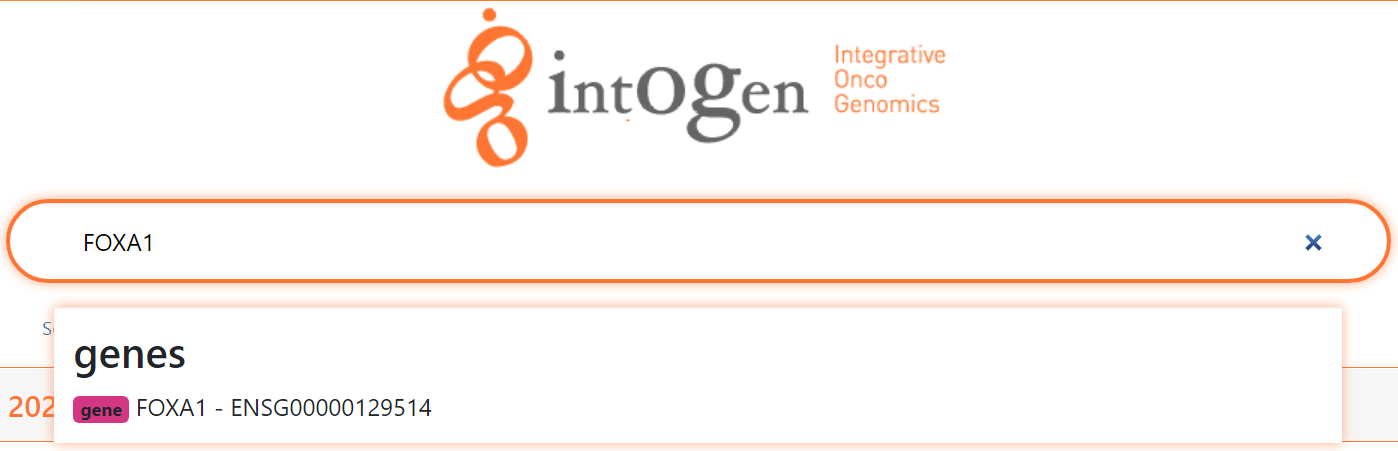
\includegraphics[width=\textwidth]{FOXA1 search.png}

  \subsection{Выбранный ген в базе данных IntOGen}
  \begin{center}
    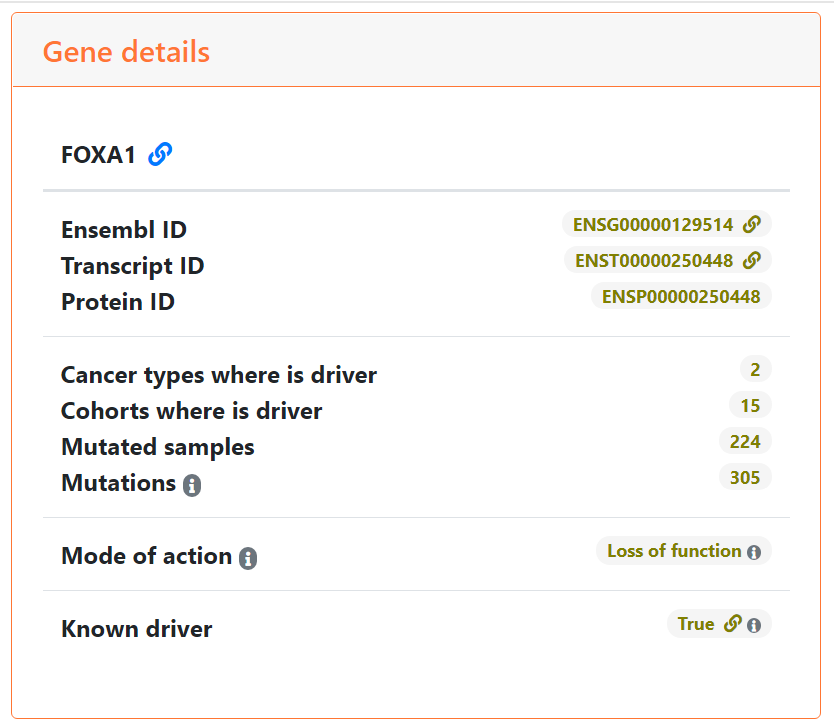
\includegraphics[width=0.5\textwidth]{gene details.png}\\
    \url{https://www.intogen.org/search?gene=FOXA1}
  \end{center}

  \subsubsection{Типы рака, в которых он мутировал}
  Prostate adenocarcinoma и Breast adenocarcinoma

  \noindent
  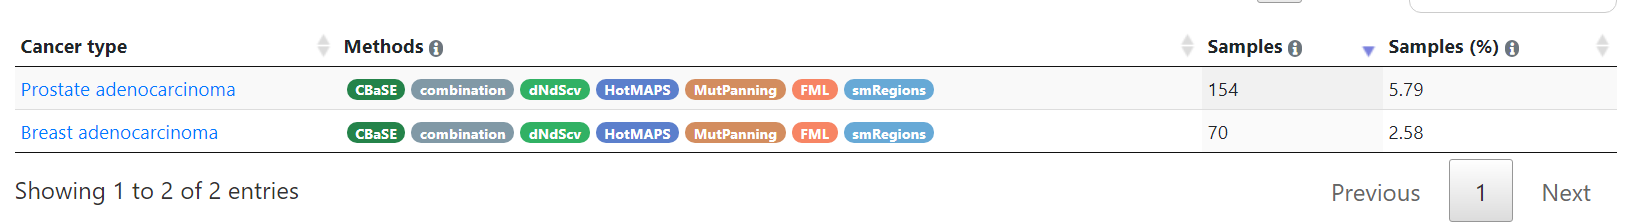
\includegraphics[width=\textwidth]{cancer types.png}

  \subsubsection{Типы мутаций}
  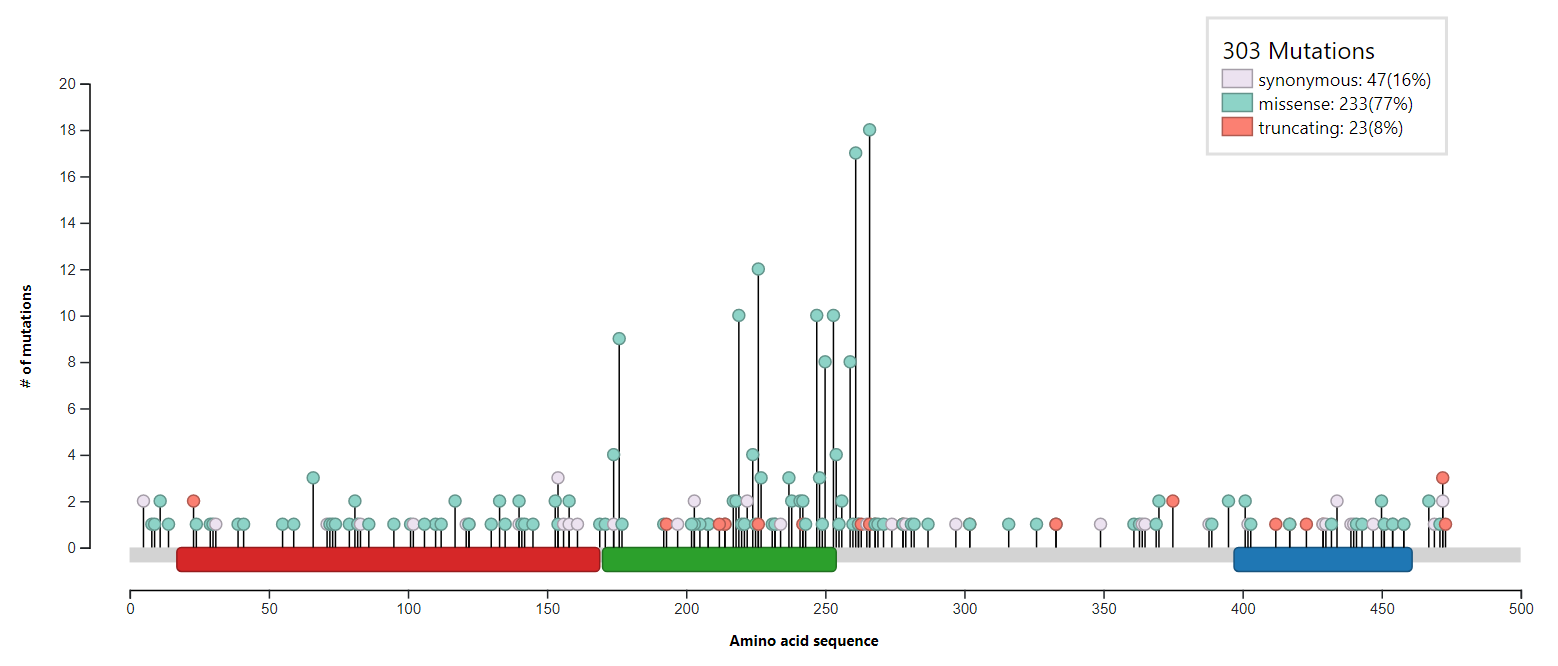
\includegraphics[width=\textwidth]{mutation plot.png}

  \noindent
  Все мутации точечные и 13 из них делиции а все остальные однонуклеотидные замены

  \noindent
  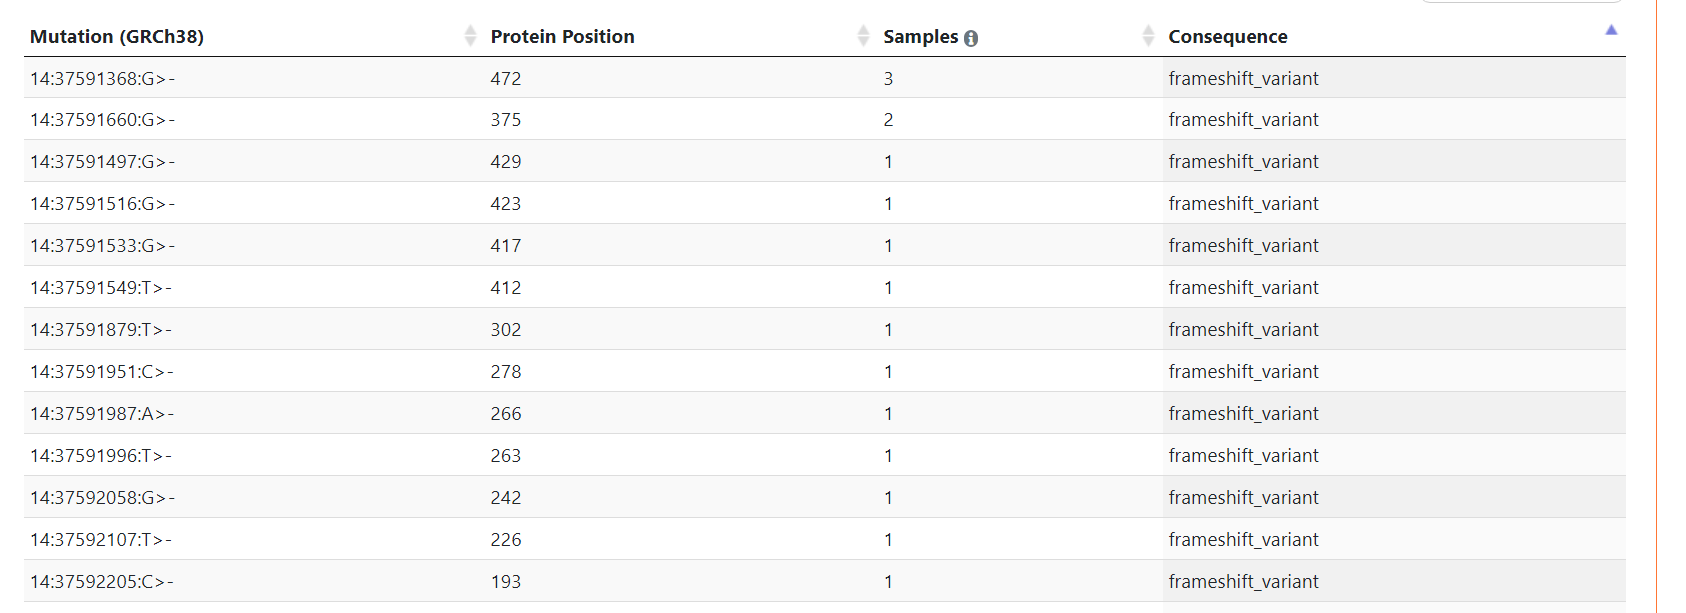
\includegraphics[width=\textwidth]{deletion mutations.png}

  \subsection{Поиск выбранного гена на портале ICGC}
  \begin{center}
    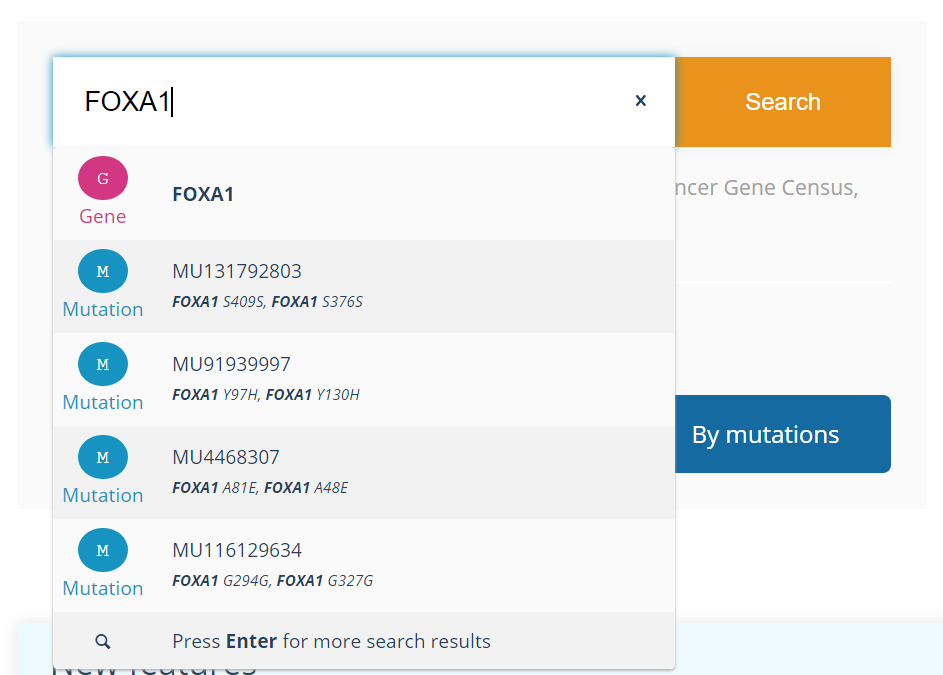
\includegraphics[width=0.5\textwidth]{search 2.png}\\
    \url{https://dcc.icgc.org/genes/ENSG00000129514}
  \end{center}

  \subsubsection{Типы рака, в которых он мутировал}
  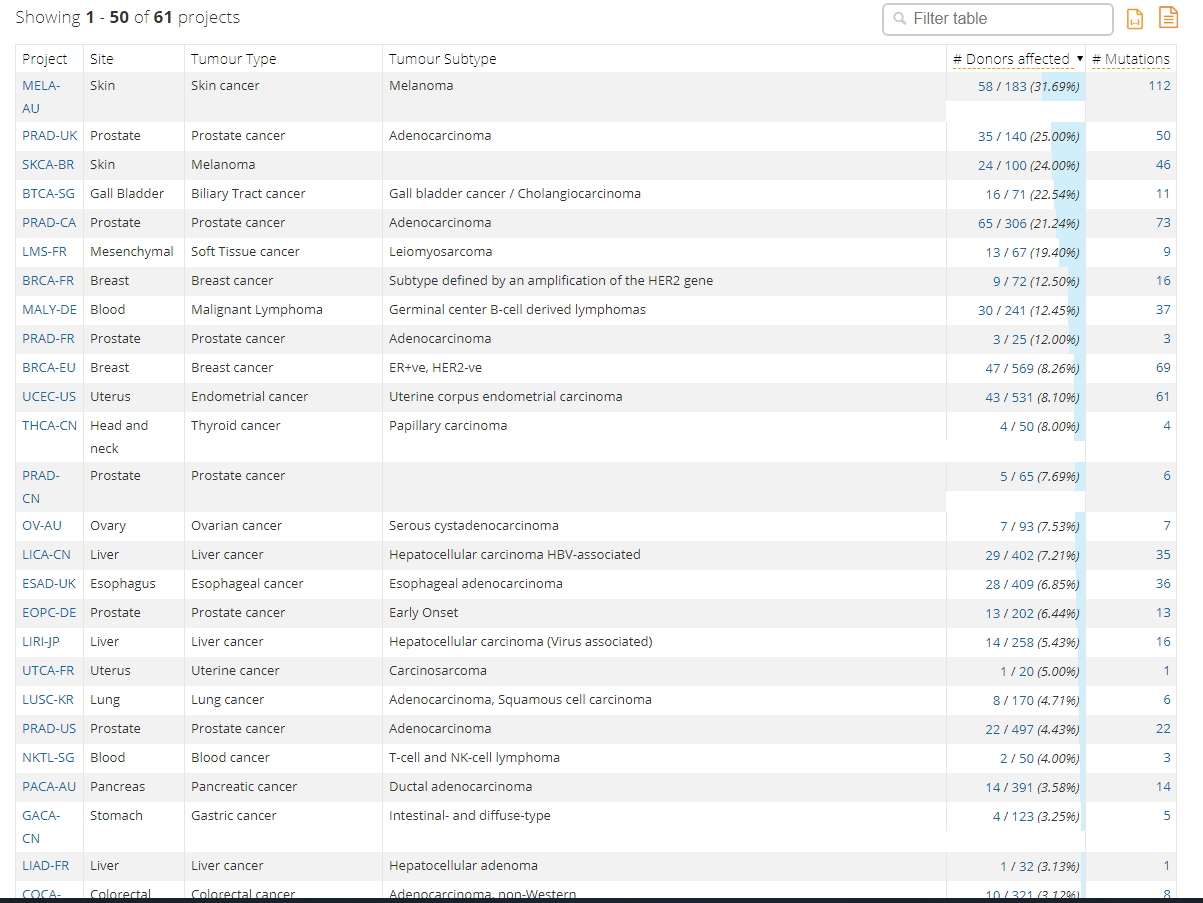
\includegraphics[width=\textwidth]{more cancer types.png}

  \newpage
  \section{Выбранный индивидуальный геном}
  \begin{center}
    \url{https://dcc.icgc.org/donors/DO218269}
  \end{center}

  \noindent
  % \begin{tabular}{p{\textwidth-6cm}r}
    В скаченном файле гены хранятся по их Ensembl ID.
    У нашего FOXA1 Ensembl ID получился ENSG00000129514.
    Мутаций в этом гене у нас нет.
    Я выбрал ещё 4 гена LRP1B, PCDH15, CSMD1 и CNTNAP2,
    потому что это гены с самым большим количеством мутации в базе данных ICGC.
    Ensembl ID у них ENSG00000168702, ENSG00000150275, ENSG00000183117 и ENSG00000174469 соответственно.
    Мутаций в них во всех есть и много.
    % &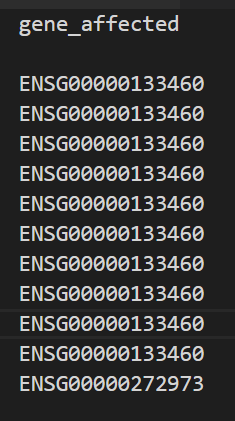
\includegraphics[align=t,width=5cm]{gene_affected.png}
  % \end{tabular}

  \begin{center}
    \begin{tabular}{|l|l|l|}
      \hline
      ген & Ensembl ID & скриншот \\\hline
      FOXA1 & \href{https://dcc.icgc.org/genes/ENSG00000129514}{ENSG00000129514} & 
\includegraphics[align=c]{ENSG00000129514.png} \\\hline
      LRP1B & \href{https://dcc.icgc.org/genes/ENSG00000168702}{ENSG00000168702} & 
\includegraphics[align=c]{ENSG00000168702.png} \\\hline
      PCDH15 & \href{https://dcc.icgc.org/genes/ENSG00000150275}{ENSG00000150275} & 
\includegraphics[align=c]{ENSG00000150275.png} \\\hline
      CSMD1 & \href{https://dcc.icgc.org/genes/ENSG00000183117}{ENSG00000183117} & 
\includegraphics[align=c]{ENSG00000183117.png} \\\hline
      CNTNAP2 & \href{https://dcc.icgc.org/genes/ENSG00000174469}{ENSG00000174469} & 
\includegraphics[align=c]{ENSG00000174469.png} \\\hline
    \end{tabular}
  \end{center}

\end{document}
